\subsection{Miller}
Il \emph{miller} è il componente che simula la fresatura vera e propria, verificando dove e come l'utensile della macchina compenetra il blocco di materiale, determinando la porzione da rimuovere e decidendo se sia o meno necessario attivare il getto d'acqua di pulitura.

Per gestire in maniera efficiente l'intero processo, si è usata come struttura dati di appoggio un octree non bilanciato, ovvero un albero di arietà 8 che, come si evince dalla figura \ref{fig:octree_explanation}, segmenta in modo efficace uno spazio tridimensionale. Ogni foglia dell'octree -rappresentante un parallelepipedo di volume detto voxel- memorizza lo stato di erosione dei propri vertici, a cui si aggiungono, per motivi di performance, le informazioni necessarie a calcolare le coordinate dei vertici stessi ed un collegamento alle strutture dati adibite alla visualizzazione grafica del blocco, come spiegato nella sezione \ref{sec:modules_mesher}.
\begin{figure}[htp]
	\centering
	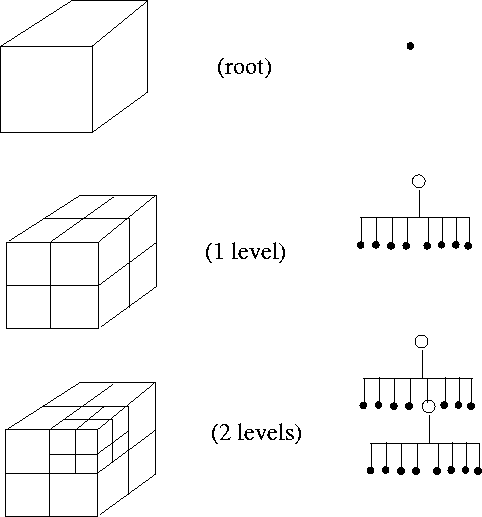
\includegraphics[width=.75\textwidth]{img/octree_explanation}
	\caption{Suddivisione dello spazio tridimensionale tramite albero octree. {\footnotesize (fonte immagine: \url{http://www.forceflow.be/wp-content/uploads/2012/04/octree1.gif})}}
	\label{fig:octree_explanation}
\end{figure}

\paragraph{Il processo di erosione.}
Per ogni ``mossa'' letta da file, il \emph{miller} converte le due rototraslazioni in una isometria tridimensionale del cutter nei confronti del sistema di riferimento del prodotto.  L'algoritmo di milling attraversa quindi l'octree per individuare tutti e soli i voxel che contengono un punto di contatto tra i due oggetti: i rami da percorrere sono scelti in base a diverse funzioni di intersezione che diventano via via meno precise, ma più veloci, man mano che aumenta la profondità e, di conseguenza, il numero di voxel da analizzare. Quando l'algoritmo giunge ad una foglia dell'albero, esso verifica se alcuni dei vertici associati risultano interni alla superficie di taglio del cutter, marcandoli come erosi. Le foglie rimaste prive di vertici vengono quindi eliminate dall'albero, mentre per le altre, se la profondità massima non è ancora stata raggiunta, l'algoritmo effettua una divisione in otto parti del volume di competenza, aggiungendo un nuovo livello all'albero. Come scelta progettuale si è deciso di non condividere i vertici comuni tra voxel contigui in quanto il concetto di vicinanza spaziale non viene modellato bene dalla struttura octree, soprattutto se sbilanciata. Il costo computazionale necessario a recuperare i voxel ``vicini'', infatti, sarebbe stato superiore ai vantaggi portati dalla condivisione dei vertici stessi. Al termine di ogni mossa, il \emph{miller} conteggia la quantità di materiale eroso e non ancora pulito e decide se attivare o meno il getto d'acqua: la scelta viene presa tramite una funzione a doppia soglia, caratterizzata da un ``rate di pulitura'', cioè dal volume di detriti che l'acqua riesce a pulire per ogni mossa.

Mostrare a video lo stato dell'erosione comporta uno scambio di informazioni tra \emph{miller} e \emph{mesher} in quanto questi due algoritmi operano in modo indipendente e con diversi tempi di elaborazione. Per gestire in maniera efficiente l'accesso concorrente ai dati, ogniqualvolta una foglia viene cancellata il \emph{miller} la inserisce in una lista opportuna mentre, per le foglie aggiunte o modificate, il percorso da esse alla radice viene evidenziato. Così facendo il processo di \emph{meshing}, dopo aver acquisito il controllo esclusivo dell'octree, potrà ricavare rapidamente tutte e sole le foglie modificate dalla sua ultima visita. Per impedire che il processo di \emph{milling} possa subire starvation dal \emph{mesher}, quest'ultimo viene attivato al più al termine di ogni mossa letta da file e, comunque, non più di 30 volte al secondo: nei casi reali il tempo di attesa forzata del \emph{miller} è ridotto in quanto, un ciclo di rendering impiega molto più tempo della simulazione di una singola posizione e quest'ultima è più lenta dell'attraversamento dell'albero sui percorsi evidenziati\footnote{I rapporti tra le durate delle operazioni indicate variano di molto in base alla profondità massima dell'albero e alla ``mobilità'' dell'utensile, ovvero al numero di voxel modificati ad ogni iterazione.}.

\paragraph{Sviluppi futuri.}
Il processo di \emph{milling} è frutto di più riscritture successive, ognuna delle quali ha sperimentato un modo diverso per rendere più efficiente e veloce l'algoritmo: la versione attuale risulta essere la più performante in single-thread ma, dal punto di vista dello spazio occupato, potrebbe essere ulteriormente migliorata sfruttando in maniera più intelligente la ricorsione\footnote{Attualmente ogni nodo dell'albero contiene un riferimento al padre, retaggio di vecchie implementazioni: questo puntatore può essere rimosso mantenendo comunque la possibilità di ``risalire'' la struttura dati, durante il completamento delle chiamate ricorsive.}. Il vero salto di qualità, però, si avrebbe rendendo multi-threaded il processo di erosione. L'esperienza da noi maturata indica che la strada da seguire per ottenere il massimo delle prestazioni è analizzare l'octree usando il pattern Fork-Join\footnote{\url{http://www.oracle.com/technetwork/articles/java/fork-join-422606.html}} congiuntamente a uno thread-pool che permetta il \emph{work-stealing}: in questo modo si conservano tutti i vantaggi della ricorsione, con l'aggiunta di quelli dovuti a un processing embarassingly parallel, in quanto i thread elaborano dati indipendenti gli uni dagli altri.
